% !TEX root = pfc.tex

Como visto no Capítulo \ref{cha:vis_o_computacional}, existem diversas técnicas de processamento digital de imagens que viabilizam a construção de sistemas de visão computacional. A Seção \ref{sec:aplica_es_de_vis_o_computacional} descreve exemplos de sistemas de visão computacional voltados para o monitoramento do tráfego, deixando claro o alto nível de complexidade dessas aplicações do ponto de vista de desenvolvimento. São trabalhos com ótimos resultados, mas de elevada complexidade algorítmica, exigindo um conhecimento profundo na área para um entendimento completo das metodologias propostas.

Este trabalho se diferencia dos demais por adotar uma metodologia simplificada, utilizando algoritmos de processamento de imagem já implementados pela biblioteca OpenCV 2.4.4 \citep{opencv_library}, diminuindo a complexidade da solução. Nas seções a seguir, o fluxo de processos é descrito e detalhado, bem como as características de captura e cena especificadas.

\section{Características de captura} % (fold)
\label{sec:caracter_sticas_de_captura}

A captura das imagens do tráfego foram feitas com a câmera que equipa um aparelho celular Samsung OMNIA W GT-I8350 \citep{omnia:2013:online}, com as seguintes especificações:

\begin{itemize}
  \item CPU: 1,4 GHz
  \item Memória: 8 GB
  \item Sistema operacional: Windows Phone 7.8
  \item Câmera: 5.0 Megapixel
  \item Gravação de vídeos HD 720p @30fps\footnote{\textit{Frames per second}, ou frames por segundo.}
\end{itemize}

Inicialmente, as imagens foram capturadas e salvas na memória interna do aparelho, e num segundo momento transferidas para um \textit{Laptop} onde seriam processadas. Todas as imagens foram capturadas durante o dia, em condições de iluminação estável e boa luminosidade. Portanto, o método proposto neste trabalho não está validado para grandes variações de iluminação ou cenas com pouca luz.

Em sistemas de monitoramento do tráfego que utilizam câmeras é muito comum a ocorrência de oclusão, ou seja, dependendo do ângulo de captura, alguns veículos não aparecem em parte ou por completo nas imagens. Alguns sistemas automáticos de contagem mais complexos tratam o problema de oclusão utilizando modelos para a forma dos veículos e calibração de câmera \citep{song:2005}. O método de contagem desenvolvido neste trabalho não considera a possibilidade de oclusão e, com intuito de minimizar esse efeito, buscou-se um ângulo de captura superior e frontal à via. Portanto, as imagens foram capturadas na passarela para pedestres localizada na Avenida Presidente Carlos Luz 3001, Pampulha, Belo Horizonte - MG, nas proximidades do Shopping Del Rey, em ambos os sentidos. A Figura \ref{fig:cena} ilustra a posição de captura e a cena obtida.

\begin{figure}[ht]
  \begin{center}
    \begin{subfigure}[b]{.49\textwidth}
      \begin{center}
        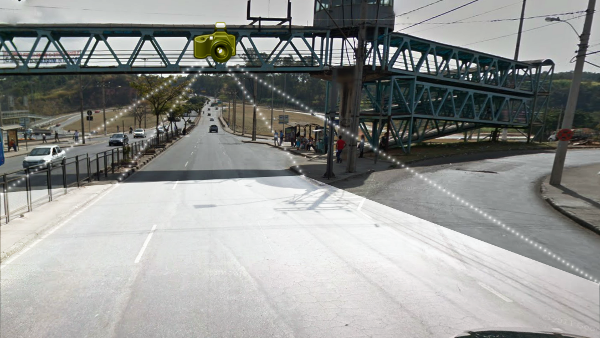
\includegraphics[width=1\linewidth]{imgs/cena_captura.png}
      \end{center}
      \caption{}
      \label{fig:cena_captura}
    \end{subfigure}
    \begin{subfigure}[b]{.49\textwidth}
      \begin{center}
        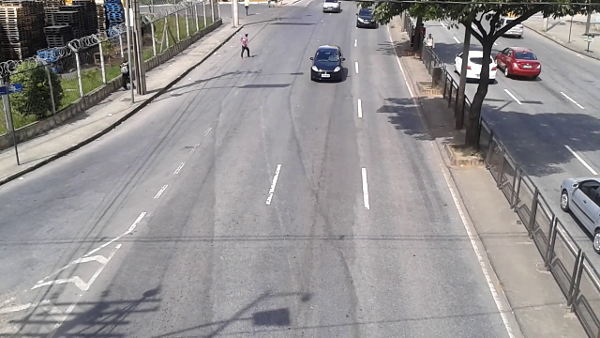
\includegraphics[width=1\linewidth]{imgs/original_frame.png}
      \end{center}
      \caption{}
      \label{fig:original_frame}
    \end{subfigure}
  \end{center}
  \caption{(a) Posicionamento da câmera para captura de imagens. A área em destaque simboliza o campo de visão obtido na posição escolhida. (b) Cena capturada na Avenida Presidente Carlos Luz no sentido Pampulha.}
  \label{fig:cena}
\end{figure}

Nas imagens capturadas pode-se perceber vários veículos de grande porte trafegando na via, como ônibus e caminhões. Esse tipo de tráfego é ainda mais comum no sentido Pampulha com presença da Fábrica da Coca-Cola ali localizada. Quando veículos grandes entram em cena é possível observar dois fenômenos que podem interferir no método de rastreamento proposto: a oclusão de veículos menores que trafegam na via no mesmo momento e a vibração da passarela quando ônibus e caminhões estão saindo de cena. Como a câmera está afixada na passarela, a vibração gera a movimentação da câmera, resultando em uma variação momentânea de enquadramento. Esse efeito, quando ocorre em um grau mais acentuado, pode causar problemas na etapa de subtração de \textit{background}, descrita a seguir na Subseção \ref{sub:subtra_o_de_background}. No entanto, tratar esse tipo de situação elevaria significativamente a complexidade do método, contrariando os objetivos inicialmente definidos.

Portanto, o método de rastreamento e contagem proposto por esse trabalho assume as seguintes premissas:

\begin{itemize}
   \item A cena possui boa iluminação, com pouca variação ao longo do tempo;
   \item Não existem oclusões parciais ou totais entre veículos;
   \item A câmera não sofre grandes vibrações ou movimentações;
   \item A contagem volumétrica não é classificatória.
 \end{itemize} 

% section caracter_sticas_de_captura (end)

\section{Fluxo de processos} % (fold)
\label{sec:fluxo_de_processos}

O método aqui apresentado pode ser dividido em seis etapas globais: entrada de dados, pré-processamento, subtração de \textit{background}, binarização, detecção de \textit{blobs} e rastreamento e contagem. A Figura \ref{fig:general_process} representa o fluxograma global do processo.

Para cada etapa de processamento de imagens existe o código \verb!C++! correspondente às operações realizadas pelas mesma, com o objetivo de mostrar a simplicidade de uso da biblioteca OpenCV. O resultado obtido em cada etapa é apresentado por meio de imagens intermediárias do processo. Na última etapa, o fluxograma da Figura \ref{fig:fluxograma_contagem} descreve o algoritmo implementado para rastreamento e contagem dos veículos.

\begin{figure}[ht]
  \begin{center}
    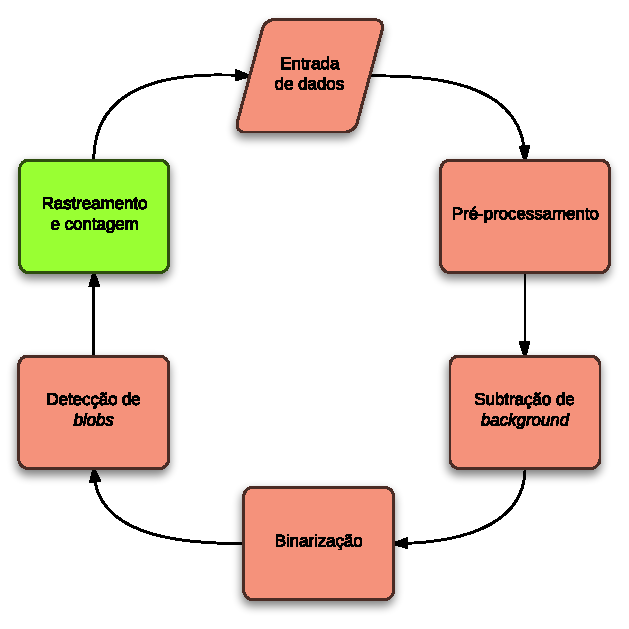
\includegraphics[scale=0.9]{imgs/general_process.pdf}
  \end{center}
  \caption{Fluxograma com a representação global do método de contagem.}
  \label{fig:general_process}
\end{figure}

De forma resumida, o método proposto considera o vídeo como um conjunto de imagens sequenciais, obtidas uma a uma na etapa de entrada de dados. Em seguida, cada imagem, chamada também de quadro ou \textit{frame} de vídeo, passa por uma etapa de pré-processamento, responsável pela conversão para escala de cinza e uma filtragem linear. O resultado é usado para criação de um modelo do plano de fundo da cena e que, por meio de uma subtração do quadro atual, consegue-se isolar os objetos em movimento que encontram-se em primeiro plano. Na etapa de binarização, um limiar de intensidade de cor segmenta a imagem em regiões brancas, que são os objetos em movimento, e pretas, que representam o plano de fundo. Posteriormente, os objetos brancos em movimento são detectados como componentes conectados ou \textit{blobs}, e seu centro é tido como ponto chave para a etapa de rastreamento e contagem. Por último, um algoritmo considera os pontos chave, ou \textit{keypoints}, para realizar o rastreamento e contagem dos veículos.

\subsection{Entrada de dados} % (fold)
\label{sub:entrada_de_dados}

A obtenção dos dados em um sistema de visão computacional pode ser feita em tempo real ou a partir de imagens já capturadas previamente. No trabalho em questão, esse processo se dá por meio de vídeos já salvos em disco, através do trecho de código \verb!C++! a seguir:

\begin{lstlisting}
#include <iostream>
#include <opencv2/core/core.hpp>
#include <opencv2/highgui/highgui.hpp>
#include <opencv2/imgproc/imgproc.hpp>

int main(int argc, char const *argv[])
{
  cv::VideoCapture capture("video.avi");
  if(!capture.isOpened()) {
    std::cout << "can not open camera or video file" << std::endl;
    return;
  }
  ...  
  for(;;) {
    cv::Mat frame;
    capture >> frame;

    if(frame.empty()) break; 
    ...  
  }

  return 0;
}
\end{lstlisting}

A classe \verb!cv::VideoCapture! da OpenCV faz todo o trabalho de obtenção dos \textit{frames}, abstraindo um arquivo de vídeo por uma sequência de imagens, obtidas uma a uma na linha: \verb!capture >> frame!. A Figura \ref{fig:frame_in} representa um \textit{frame} do vídeo, usado para exemplificar o resultado do processamento de cada etapa subsequente. 

Vale ressaltar que a biblioteca OpenCV utiliza objetos do tipo \verb!cv::Mat! para armazenar em memória os dados de uma imagem, sendo este também o tipo de entrada e saída para a maioria das funções de processamento de imagem.

\begin{figure}[ht]
  \begin{center}
    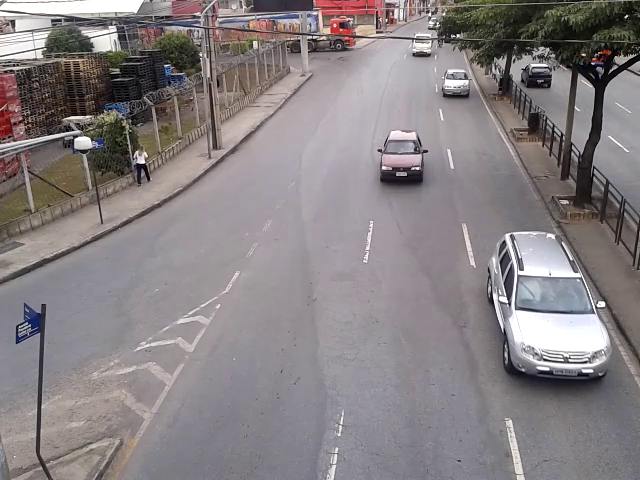
\includegraphics[scale=0.5]{imgs/frame.png}
  \end{center}
  \caption{\textit{Frame} obtido a partir do vídeo de entrada.}
  \label{fig:frame_in}
\end{figure}

% subsection entrada_de_dados (end)

\subsection{Pré-processamento} % (fold)
\label{sub:pr_processamento}

A principal função da etapa de pré-processamento é a conversão da imagem de entrada para \textit{grayscale}, uma vez que informações de cor não são relevantes nas etapas seguintes e o processamento de imagens em escala de cinza, que possuem apenas um canal, é mais rápido. No código, a conversão é feita pela chamada da função \verb!cv::cvtColor!, passando como parâmetros as imagens de entrada e saída, e o \textit{flag} \verb!CV_BGR2GRAY!, que indica o tipo de operação desejada.

\begin{lstlisting}
  ...
  for(;;) {
    ...
    cv::Mat gray;
    cv::cvtColor(frame, gray, CV_BGR2GRAY);

    cv::GaussianBlur(gray, gray, cv::Size(7, 7), 3);
    ...
  }
  ...  
\end{lstlisting}

Em seguida, utiliza-se uma filtragem linear gaussiana, descrita na Seção \ref{sec:filtragem_linear}, com o objetivo de atenuar ruídos oriundos do processo de captura e provocar um efeito suave de borramento na imagem. Esse processo diminui as componentes de alta frequência presentes entre um \textit{frame} e outro, que podem interferir na etapa de subtração de \textit{background} descrita a seguir na Subseção \ref{sub:subtra_o_de_background}. 

A chamada da função \verb!cv::GaussianBlur! realiza a operação de filtragem, que é parametrizada pelas imagens de entrada e saída, o tamanho do \textit{kernel} utilizado como elemento de convolução e o desvio padrão nas direções X e Y. O resultado desse procedimento é ilustrado na Figura \ref{fig:pre_processamento}.

\begin{figure}[ht]
  \begin{center}
    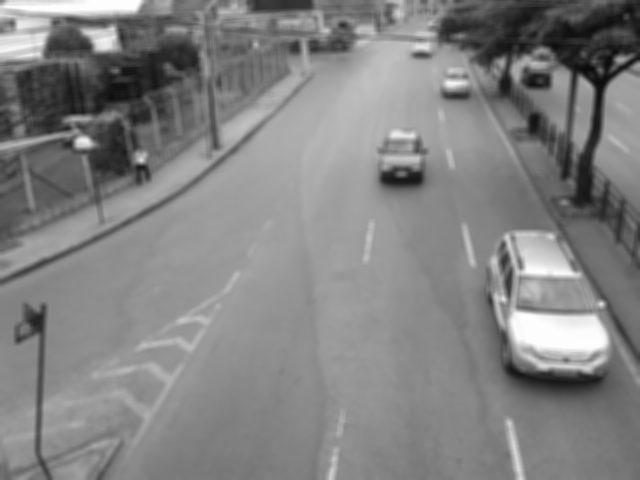
\includegraphics[scale=0.5]{imgs/gray.png}
  \end{center}
  \caption{Resultado da etapa de pré-processamento, uma imagem filtrada em escala de cinza.}
  \label{fig:pre_processamento}
\end{figure}

% subsection pr_processamento (end)

\subsection{Subtração de \textit{background}} % (fold)
\label{sub:subtra_o_de_background}

A subtração de \textit{background} é a operação mais complexa e custosa, do ponto de vista computacional, entre todas as etapas de processamento de imagens do trabalho em questão, mas o seu uso, a partir da implementação da OpenCV, é extremamente simples. Internamente, a OpenCV constrói um modelo adaptativo de mistura de gaussianas para subtração de \textit{background} com detecção de sombras, baseado em \cite{zivkovic:2004} e \cite{zivkovic:2006}. Nesse método, cada píxel é modelado como uma mistura de gaussianas e, em cada iteração, a probabilidade do pixel pertencer ao plano de fundo é calculada.

\begin{lstlisting}
  ...
  cv::BackgroundSubtractorMOG2 model;
  for(;;) {
    ...
    cv::Mat foreground;
    model(gray, foreground);
    ...
  }
  ...
\end{lstlisting}

No código \verb!C++!, essa operação pode ser realizada em duas linhas: a declaração do objeto \verb!model! da classe \verb!cv::BackgroundSubtractorMOG2! e a extração da imagem de \textit{foreground}, ou imagem de primeiro plano, com a chamada \verb!model(gray, foreground)!. O resultado é mostrado na Figura \ref{fig:foreground}, onde os pixels pretos representam o plano de fundo, os brancos os objetos em movimento do primeiro plano e os pixels cinza suas sombras.

\begin{figure}[ht]
  \begin{center}
    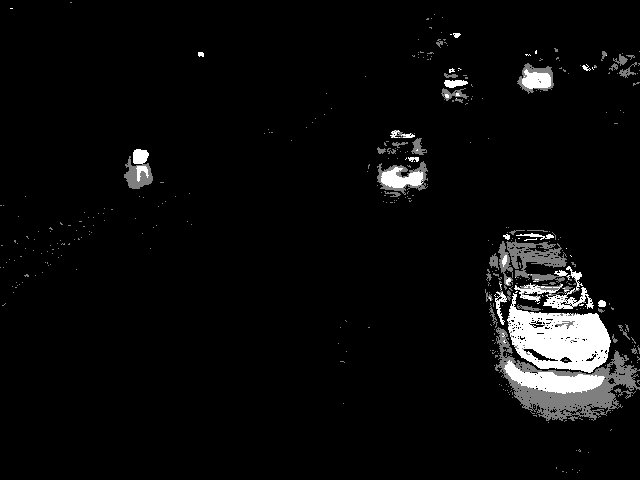
\includegraphics[scale=0.5]{imgs/foreground.png}
  \end{center}
  \caption{Detecção do \textit{foreground} na etapa de subtração de fundo.}
  \label{fig:foreground}
\end{figure}

% subsection subtra_o_de_background (end)

\subsection{Binarização} % (fold)
\label{sub:binariza_o}

Em visão computacional, imagens binárias são aquelas que possuem apenas dois valores de intensidade, normalmente 0 (preto) e 255 (branco). Geralmente, os pixels brancos pertencem aos objetos de interesse da cena, que no escopo desse trabalho fazem parte dos veículos em movimento. A etapa de binarização é responsável por segmentar as regiões de interesse da cena para que, nas próximas etapas, sejam detectadas e rastreadas.

A imagem de primeiro plano obtida na etapa anterior (Subseção \ref{sub:subtra_o_de_background}) possui pixels cinza, que representam as sombras dos objetos. Analisando a Figura \ref{fig:foreground}, percebe-se que os pixels brancos sozinhos não definem muito bem um veículo, mas o conjuntos dos pixels branco e cinza sim. Então, é feita uma operação de limiarização, também conhecida por \textit{thresholding} (Seção \ref{sec:limiariza_o}), com intuito de elevar o valor de todos os pixels cinza para branco. Isso é feito pela chamada da função \verb! cv::threshold!, parametrizada pelas imagens de entrada e saída, um valor de limiar baixo, que garante a elevação à branco de praticamente todos os tons de cinza, e o tipo de limiarização a ser aplicada, nesse caso binária. 

Percebe-se na Figura \ref{fig:bin} que a operação de \textit{thresholding} segmentou corretamente os veículos. No entanto, para detecção de objetos em visão computacional, é interessante que as regiões de interesse sejam uniformes e não contenham orifícios. Nesse tipo de situação é comum o uso de operações morfológicas, capazes de alterar a forma dos objetos segmentados em imagens binárias. Como o objetivo é uniformizar a região de segmentação dos objetos, deve-se aplicar uma operação de fechamento, que diminui orifícios e descontinuidades nas regiões de interesse, alongando os segmentos de cor branca pelas imperfeições de cor preta. A Figura \ref{fig:morph} mostra uma melhor uniformidade na região dos objetos segmentados.

\begin{lstlisting}
  ...
  for(;;) {
    ...
    cv::threshold(foreground, foreground, 5, 255, CV_THRESH_BINARY);

    cv::Mat morph;
    cv::Mat element = cv::getStructuringElement(cv::MORPH_ELLIPSE,
                                                cv::Size(5,5));
    cv::morphologyEx(foreground, morph, CV_MOP_CLOSE, element, 
                     cv::Point(-1,-1), 3);
    ...
  }
  ...  
\end{lstlisting}

As operações morfológicas, assim como os filtros, também utilizam um elemento estrutural que percorre toda a imagem. Nesse caso, utilizou-se um \textit{kernel} elíptico, que é a forma que mais se aproxima de um veículo na imagem binarizada. A criação desse elemento se dá pela chamada da função \verb!cv::getStructuringElement!, que recebe como parâmetro a forma e o tamanho desejados. A operação de fechamento propriamente dita é feita pelo método \verb!cv::morphologyEx!, parametrizado pelas imagens de entrada e saída, o tipo de operação morfológica, o elemento estrutural, o ponto de ancoragem com o \textit{kernel} (\verb!cv::Point(-1,-1)!  representa o centro) e o número de iterações.

\begin{figure}[ht]
  \begin{center}
    \begin{subfigure}[b]{.49\textwidth}
      \begin{center}
        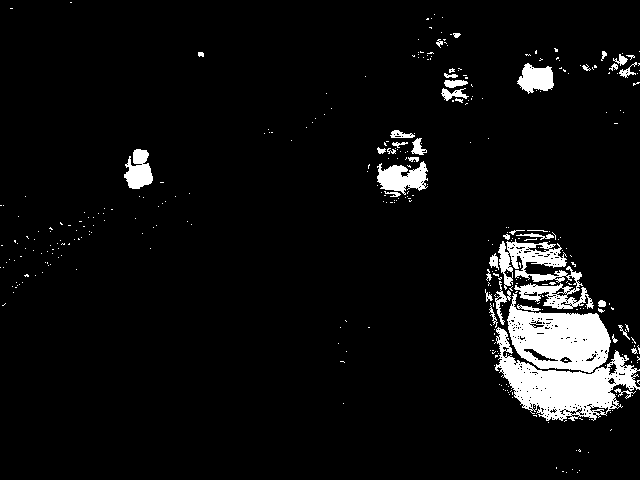
\includegraphics[width=1\linewidth]{imgs/bin.png}
      \end{center}
      \caption{}
      \label{fig:bin}
    \end{subfigure}
    \begin{subfigure}[b]{.49\textwidth}
      \begin{center}
        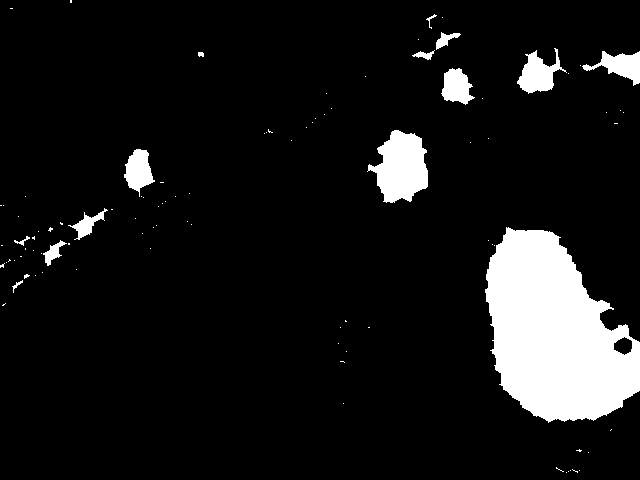
\includegraphics[width=1\linewidth]{imgs/morph.png}
      \end{center}
      \caption{}
      \label{fig:morph}
    \end{subfigure}
  \end{center}
  \caption{Resultado da etapa de binarização. (a) Imagem binarizada utilizando um limiar simples; (b) Operação morfológica de fechamento.}
  \label{fig:bin_morph}
\end{figure}

% subsection binariza_o (end)

\subsection{Detecção de \textit{blobs}} % (fold)
\label{sub:detec_o_de_blobs}

Uma vez segmentados, os objetos de interesse são detectados nessa etapa como \textit{blobs}, que são regiões de pontos com valor 255 (branco), conectados entre si, definidas pelo seu ponto central e diâmetro. A biblioteca OpenCV utiliza a entidade \verb!cv::KeyPoint! para representá-los. Nesse caso, a principal função dos \textit{keypoints} é definir a posição e tamanho de cada objeto segmentado, para que na próxima etapa esses pontos sejam rastreados pelos \textit{trackers}.

A OpenCV disponibiliza uma interface abstrata para detecção de \textit{keypoints}, chamada \verb!cv::FeatureDetector!. Uma de suas especializações é a classe \verb!cv::SimpleBlobDetector!, capaz de extrair \textit{blobs} de uma imagem. Em sua contrução, a classe \verb!cv::SimpleBlobDetector! recebe uma estrutura de parâmetros de filtragem, responsáveis por descartar pontos que não atendam as especificações desejadas. O método proposto habilita apenas dois tipos de filtro: de cor, que considera apenas \textit{blobs} brancos, e área, que abrange regiões com área mínima de 500 pixels e máxima de 80000.

\begin{lstlisting}
  ...
    cv::SimpleBlobDetector::Params params;
    params.filterByInertia = false;
    params.filterByConvexity = false;
    params.filterByColor = true;
    params.blobColor = 255;
    params.filterByCircularity = false;
    params.filterByArea = true;
    params.minArea = 500.0f;
    params.maxArea = 80000.0f;

    cv::Ptr<cv::FeatureDetector> detector = 
                                 new cv::SimpleBlobDetector(params);
    detector->create("SimpleBlob");
    ...
    for(;;) {
      ...
      std::vector<cv::KeyPoint> keypoints;
      detector.detect(morph, keypoints)
    }
    ...  
\end{lstlisting}

Uma vez criado, o objeto \verb!detector!, através do método \verb!detect!, recebe como parâmetro a imagem binarizada da Figura \ref{fig:morph} e retorna um vetor de \textit{keypoints}, contendo todos os \textit{blobs} detectados naquele \textit{frame}. A Figura \ref{fig:keypoints} ilustra os pontos detectados, representados pelos pequenos círculos indicados. 

Esta é a última operação que envolve processamento de imagem. Com a posição e o tamanho dos \textit{blobs} detectados, definidos por um vetor de \textit{keypoints}, é possível criar um algoritmo de rastreamento que garanta que cada objeto seja contado apenas uma vez, como descrito logo a seguir na Subseção \ref{sub:rastreamento_e_contagem}.

\begin{figure}[ht]
  \begin{center}
    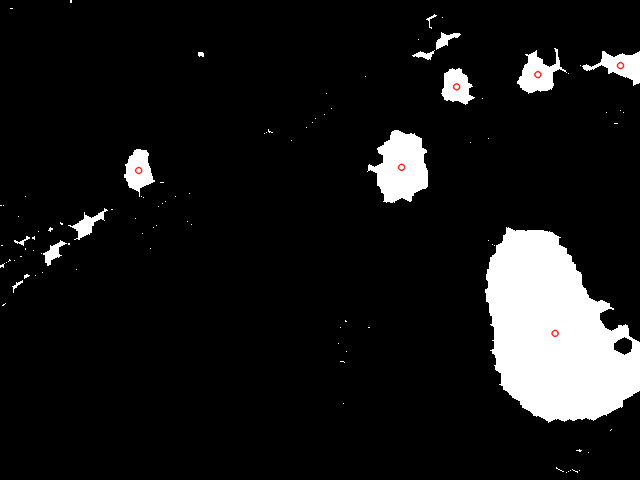
\includegraphics[scale=0.5]{imgs/keypoints.png}
  \end{center}
  \caption{Resultado da etapa de detecção de \textit{blobs}.}
  \label{fig:keypoints}
\end{figure}

% subsection detec_o_de_blobs (end)

\subsection{Rastreamento e contagem} % (fold)
\label{sub:rastreamento_e_contagem}

Assim como em todas as etapas anteriores, buscou-se a implementação de um método simples de rastreamento e contagem, mas que fosse capaz de obter bons resultados. O algoritmo utiliza o vetor de \textit{keypoints}, obtido na etapa anterior, e uma máscara binária, que define a região de contagem. Um objeto só é contabilizado quando o \textit{keypoint} que o define entra na região de contagem, definida pelos pixels brancos da Figura \ref{fig:bin_mask}.

\begin{figure}[ht]
  \begin{center}
    \begin{subfigure}[b]{.49\textwidth}
      \begin{center}
        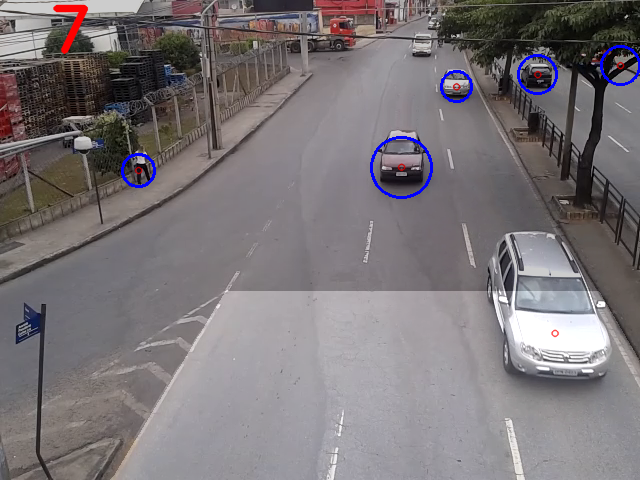
\includegraphics[width=1\linewidth]{imgs/trackers.png}
      \end{center}
      \caption{}
      \label{fig:trackers}
    \end{subfigure}
    \begin{subfigure}[b]{.49\textwidth}
      \begin{center}
        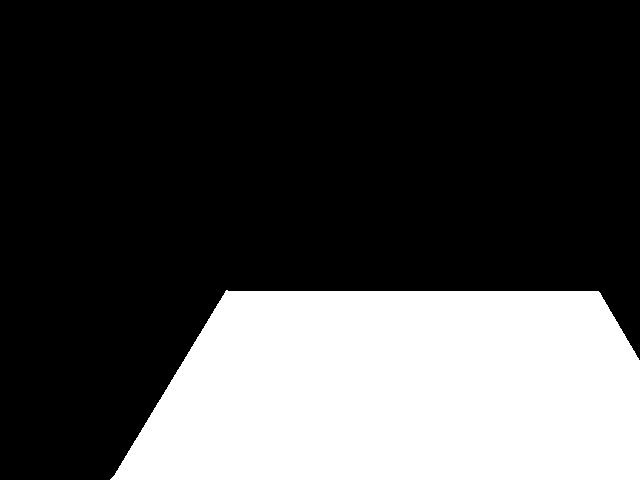
\includegraphics[width=1\linewidth]{imgs/bin_mask.png}
      \end{center}
      \caption{}
      \label{fig:bin_mask}
    \end{subfigure}
  \end{center}
  \caption{(a) Resultado da etapa de rastreamento e contagem, ilustrando \textit{trackers}, \textit{keypoints} e a região de contagem. (b) Máscara binária que define a região de contagem do algoritmo.}
  \label{fig:resultado_contagem}
\end{figure}

% \begin{figure}[ht]
%   \begin{center}
%     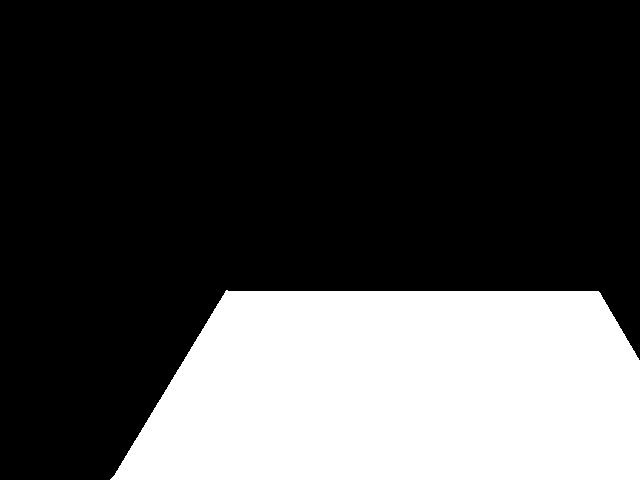
\includegraphics[scale=0.5]{imgs/bin_mask.png}
%   \end{center}
%   \caption{Máscara binária que define a região de contagem do algoritmo.}
%   \label{fig:bin_mask}
% \end{figure}

O rastreamento dos \textit{blobs}, aqui representados por \textit{keypoints}, é feito por um rastreador, denominado \textit{tracker}. Um \textit{tracker} é um objeto circular, definido por sua posição e raio. Um \textit{keypoint} está contido em um \textit{tracker} se a distância entre eles for menor que o raio do \textit{tracker}, ou seja, se o \textit{keypoint} pertencer à área definida pelo \textit{tracker}. Na Figura \ref{fig:trackers}, o \textit{tracker} é representado pelos círculos maiores. Para que um \textit{keypoint} seja contabilizado na contagem ele deve, além de ingressar na região de contagem, ser contido por pelo menos um \textit{tracker}. Internamente, o algoritmo armazena uma lista com todos os \textit{trackers} válidos, para que na próxima iteração esses dados sirvam como validação para a operação de contagem.

O fluxograma da Figura \ref{fig:fluxograma_contagem} ilustra os passos do algoritmo de rastreamento e contagem. Pra cada \textit{frame} processado é gerada uma lista de \textit{keypoints}, que tem seus itens percorridos individualmente. Para cada \textit{keypoint}, obtêm-se todos os \textit{trackers} que o contenham. Nesse momento, três situações podem ser identificadas:

\begin{enumerate}
  \item Ainda não existe nenhum \textit{tracker} que contenha \textit{keypoint};
  \item Existe apenas um \textit{tracker} que contenha \textit{keypoint};
  \item Existe mais de um \textit{tracker} que contenha \textit{keypoint}.
\end{enumerate}

\begin{figure}[ht]
  \begin{center}
    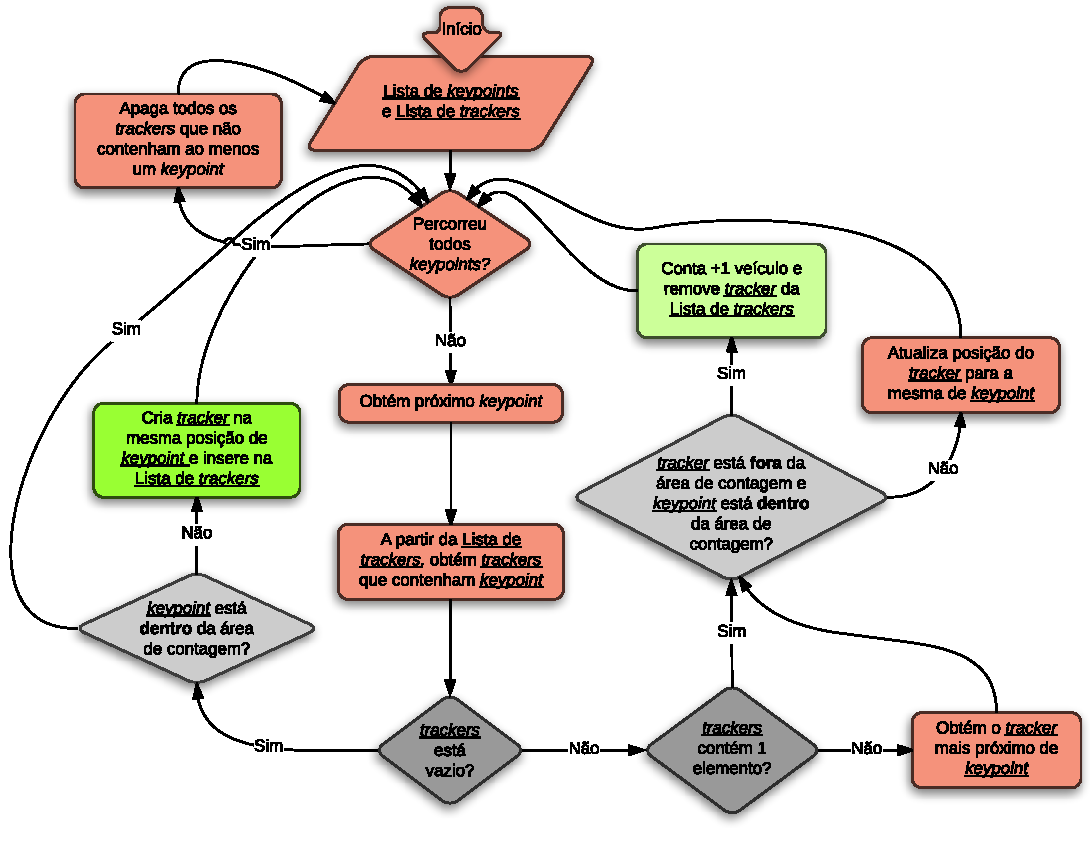
\includegraphics[scale=0.85]{imgs/fluxograma_contagem.pdf}
  \end{center}
  \caption{Fluxograma do algoritmo de rastreamento e contagem de veículos.}
  \label{fig:fluxograma_contagem}
\end{figure}

O primeiro caso acontece quando um \textit{keypoint} acabou de ser detectado na cena. Um \textit{tracker} para rastreá-lo é criado na mesma posição de \textit{keypoint} e inserido na lista interna de \textit{trackers}, a menos que o \textit{keypoint} encontre-se na área de contagem. Ou seja, não faz sentido rastrear objetos que surgiram subtamente dentro da área de contagem.

Na situação 2, o \textit{tracker} encontrado indica que o \textit{keypoint} já estava sendo rastreado nas iterações anteriores. A posição do \textit{tracker} representa exatamente a posição do objeto na última iteração. Logo, se o \textit{tracker} encontra-se \textbf{fora} da área de contagem e o \textit{keypoint} \textbf{dentro}, significa que o objeto acabou de entrar em uma condição válida de contagem, ou seja, ingressou na região de contagem definida pela máscara binária, e mais um veículo é contabilizado. Uma vez contado, o \textit{tracker} daquele objeto é removido da lista de \textit{trackers}, uma vez que não é mais necessário rastreá-lo. Caso a condição de contagem não seja atendida, a posição do \textit{tracker} é atualizada para a mesma de \textit{keypoint}.

A situação 3 acontece quando um \textit{keypoint} está contido em mais de um \textit{tracker}, devido à proximidade de dois ou mais objetos detectados na cena. Esse caso é tratado da mesma forma que na situação 2, adicionando apenas uma etapa inicial que identifica qual o \textit{tracker} mais relevante para \textit{keypoint} dentre os selecionados, ou seja, o \textit{tracker} mais próximo de \textit{keypoint}.

% \begin{figure}[ht]
%   \begin{center}
%     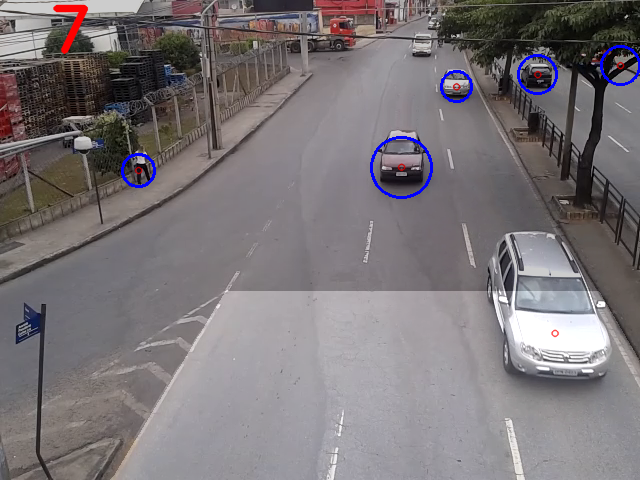
\includegraphics[scale=0.5]{imgs/trackers.png}
%   \end{center}
%   \caption{Resultado da etapa de rastreamento e contagem, ilustrando \textit{trackers}, \textit{keypoints} e a região de contagem.}
%   \label{fig:trackers}
% \end{figure}

Depois de percorrer todos os \textit{keypoints}, o algoritmo remove da lista os \textit{trackers} que não contenham ao menos um \textit{keypoint}. Isso é necessário pois a detecção de objetos não é perfeita, ou seja, se em algum \textit{frame} um objeto já anteriormente rastreado não for detectado como um \textit{keypoint}, aparece na lista de \textit{trackers} um elemento que não contém um \textit{keypoint}, configurando uma condição inválida.

A Figura \ref{fig:trackers} ilustra um veículo que entrou na região de contagem, teve seu \textit{tracker} removido e foi contabilizado corretamente. Percebe-se também que outros objetos em movimento são detectados e rastreados, como uma pessoa caminhando. No entanto, somente objetos que possuam um \textit{keypoint} contido por um \textit{tracker} e que entrem na região de contagem são contabilizados.

% subsection rastreamento_e_contagem (end)

% section fluxo_de_processos (end)

\section{Estrutura do \textit{software}} % (fold)
\label{sec:estrutura_do_software}

Para que o método aqui proposto pudesse ser testado e validado foi desenvolvido um \textit{software} multiplataforma na linguagem  \verb!C++! \citep{cplusplus:2013:online}, com intuito de obter um bom desempenho computacional, fácil implementação e a possibilidade de utilizar os conceitos de programação orientada a objetos. A Figura \ref{fig:uml} ilustra a estrutura e o relacionamento entre classes através de um diagrama de classes na notação UML\footnote{\textit{Unified Modeling Language} - um conjunto padronizado de diagramas com notação formalmente definida, adotado na área de engenharia de software em um esforço para facilitar a concepção de sistemas orientados a objetos \citep{aguiar2008thesis}.}.

\begin{figure}[ht]
  \begin{center}
    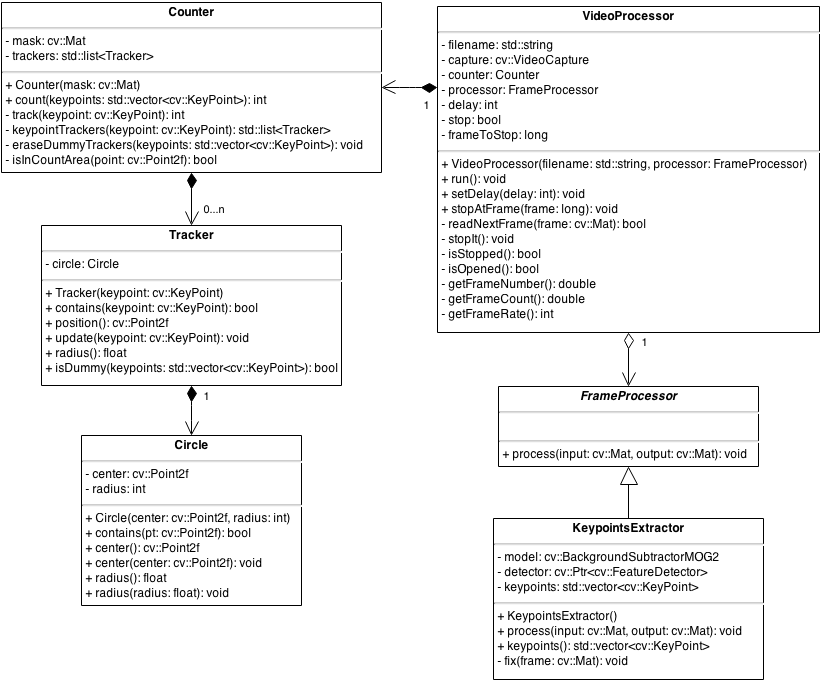
\includegraphics[scale=0.55]{imgs/uml_pfc.png}
  \end{center}
  \caption{Diagrama de classes do \textit{software}.}
  \label{fig:uml}
\end{figure}

A classe \verb!VideoProcessor! é a classe central do sistema. Ela é responsável por abrir e ler o arquivo de vídeo através do objeto \verb!capture! do tipo \verb!cv::VideoCapture!; interfacear com a classe abstrata \verb!FrameProcessor! através da chamada do método \verb!process!; e executar o algoritmo de rastreamento e contagem implementado pela classe \verb!Counter!.

A classe abstrata \verb!FrameProcessor! define uma interface cuja função é receber uma imagem de entrada, executar algum processamento sobre ela e disponibilizar o resultado. A classe \verb!KeypointsExtractor! implementa essa interface abstrata com as operações descritas nas seguintes subseções: \nameref{sub:entrada_de_dados}, \nameref{sub:pr_processamento}, \nameref{sub:subtra_o_de_background}, \nameref{sub:binariza_o} e \nameref{sub:detec_o_de_blobs}. Ou seja, essa classe concentra todas as operações de visão computacional e, através do método \verb!keypoints!, retorna os pontos que pontencialmente representam veículos em movimento.

A classe \verb!Counter! implementa o algoritmo descrito na Subseção \ref{sub:rastreamento_e_contagem}. Utilizando os \textit{keypoints}, uma máscara binária que define a região de contagem e uma lista interna de \textit{trackers}, o método \verb!count! retorna quantos eventos de contagem ocorrem para cada iteração.

A classe \verb!Circle! é utilizada pela classe \verb!Tracker! para representar um círculo com centro e raio definidos. Já a classe \verb!Tracker! é utilizada na forma de lista pela classe \verb!Counter!, na implementação do algoritmo de rastreamento e contagem.

O código dessa aplicação pode ser encontrado no seguinte repositório: \url{https://github.com/arthurbailao/potential-ironman}.

% section estrutura_do_software (end)

\section{Avaliação dos resultados} % (fold)
\label{sec:avalia_o_dos_resultados}

Para avaliar o método de rastreamento e contagem de veículos aqui proposto foram utilizadas algumas métricas já conhecidas na literatura. Nas subseções a seguir são descritas as métricas de análise de resultados usadas nesse trabalho.

\subsection{Matriz de confusão} % (fold)
\label{sub:matriz_de_confus_o}

A matriz de confusão contém informações sobre classificações reais e preditas feitas por um classificador, como mostrado na Tabela \ref{tab:matriz_de_confusao}. Ela permite que a partir de seus elementos diversas medidas de desempenho sejam calculadas.

\begin{table}[ht]
  \caption{Matriz de confusão para um classificador de duas classes.}
  \label{tab:matriz_de_confusao}
  \begin{center}
    \begin{tabular}{l|l|c|c|l}

    \multicolumn{2}{c}{} & \multicolumn{2}{c}{Classe verdadeira} & \\
    \cline{3-4}
    \multicolumn{2}{c|}{} & Positivo & Negativo & \\
    \cline{2-4}
    \multirow{2}{*}{Classe predita} & Positivo & VP & FP & Positivos previstos\\
    \cline{2-4}
    & Negativo & FN & VN & Negativos previstos \\
    \cline{2-4}
    \multicolumn{2}{c}{} & \multicolumn{1}{c}{Positivos reais} & \multicolumn{1}{c}{Negativos reais} & \\
    
    \end{tabular}
  \end{center}
\end{table}

Um verdadeiro positivo (VP) é um evento predito como pertencente à classe positiva, sendo este realmente pertencente à classe positiva. Um falso negativo (FN) acontece quando o evento predito como pertencente à classe negativa pertence à classe positiva. Analogamente, o verdadeiro negativo (VN) é um evento da classe negativa predito corretamente e o falso positivo (FP) um evento da classe negativa predito de forma incorreta.

A primeira coluna da matriz representa os eventos verdadeiramente pertencentes à classe positiva (positivos reais) e a segunda coluna os verdadeiramente pertencentes à classe negativa (negativos reais). Analogamente, a primeira linha da matriz de confusão representa os eventos que foram previstos como positivos (positivos previstos) e a segunda linha os previstos como negativos (negativos previstos).

Para evitar o viés estatístico na montagem da matriz de confusão ao caracterizar as quatro possibilidades, estabelece-se uma janela de tempo baseada no tempo médio em que um veículo leva para percorrer toda a cena, dada uma determinada condição de tráfego. A contagem pura e simples, sem considerar esta janela de tempo, levaria à não consideração dos eventos vendadeiro negativo VN. Dessa forma, os elementos da matriz de confusão podem ser descritos como:

\begin{itemize}
  \item Verdadeiro positivo (VP): mais um veículo foi contabilizado quando o mesmo adentrou a região de contagem em uma janela de tempo;
  \item Falso negativo (FN): mais um veículo não foi contabilizado quando o mesmo adentrou a região de contagem em uma janela de tempo;
  \item Verdadeiro negativo (VN): mais um veículo não foi contabilizado quando nenhum veículo adentrou a região de contagem em uma janela de tempo;
  \item Falso positivo (FP): mais um veículo foi contabilizado quando nenhum veículo adentrou a região de contagem em uma janela de tempo.
\end{itemize}

Vale ressaltar que dentro de uma janela de tempo pode acontecer um ou mais eventos, sejam eles do mesmo tipo ou não. A única restrição é que, para cada janela, no mínimo um evento deve obrigatoriamente acontecer. Na prática o evento verdadeiro negativo VN ocorre apenas quando nenhum dos outros três eventos acontece.

Algumas medidas de desempenho podem ser calculadas a partir dos elementos da matriz de confusão. São elas: Especificidade E (Equação \ref{eq:especificidade}), Valor Preditivo Negativo VPN (Equação \ref{eq:valor_preditivo_negativo}), Precisão P (Equação \ref{eq:precisao}), \textit{Recall} R (Equação \ref{eq:recall}), Acurácia A (Equação \ref{eq:acuracia}) e \textit{F-Measure} FM (Equação \ref{eq:f_measure}) \citep{powers07evaluation}.

\begin{equation}
  \label{eq:especificidade}
  E=\dfrac{VN}{VN+FP}
\end{equation}

\begin{equation}
  \label{eq:valor_preditivo_negativo}
  VPN=\dfrac{VN}{VN+FN}
\end{equation}

\begin{equation}
  \label{eq:precisao}
  P=\dfrac{VP}{VP+FP}
\end{equation}

\begin{equation}
  \label{eq:recall}
  R=\dfrac{VP}{VP+FN}
\end{equation}

\begin{equation}
  \label{eq:acuracia}
  A=\dfrac{VP+VN}{VP+FP+FN+VN}
\end{equation}

\begin{equation}
  \label{eq:f_measure}
  FM=\dfrac{2*R*P}{R+P}
\end{equation}

A Precisão representa a proporção dos eventos positivos previstos que são positivos reais. O índice \textit{Recall} é a proporção dos positivos reais que são previstos como positivos \citep{powers07evaluation}. Seguindo o mesmo raciocínio, Especificidade é a proporção dos eventos negativos reais que são previstos como negativos e Valor Preditivo Negativo a proporção dos eventos negativos previstos que são negativos reais. A Acurácia representa o percentual de eventos acertivos, considerando todos os elementos da matriz de confusão. E o índice \textit{F-Measure} é definido como a média harmônica da Precisão e \textit{Recall}, no qual um valor alto indica valores altos de ambas parcelas \citep{dener:2013}.

% subsection matriz_de_confus_o (end)

\subsection{Índice Kappa (K)} % (fold)
\label{sub:_ndice_kappa_}

O índice Kappa é utilizado como uma medida apropriada da exatidão por representar inteiramente a matriz de confusão. Ele toma todos os elementos da matriz ao invés de apenas aqueles que retratam a quantidade de classificações verdadeiras, o que ocorre quando se calcula a exatidão global da classificação \citep{Jnl605963009}. Segundo \cite{Anthony2005}, o índice Kappa é uma medida de concordância entre avaliadores, muito utilizada em estudos da área médica. No contexto desse trabalho ele representa o nível de concordância entre uma contagem manual referência e a contagem automática, gerando uma medida capaz de avaliar a qualidade do método proposto.

O índice Kappa pode ser encontrado com base na Equação \ref{eq:kappa}:

\begin{equation}
  \label{eq:kappa}
  K=\dfrac{\theta_{1}-\theta_{2}}{1-\theta_{2}}\text{,}
\end{equation}

\noindent onde

\begin{equation}
  \label{eq:theta_1}
  \theta_{1}=\dfrac{VP+VN}{VP+FP+FN+VN}
\end{equation}

\noindent e

\begin{equation}
  \label{eq:theta_2}
  \theta_{2}=\dfrac{\alpha+\beta}{\gamma^{2}}\text{,}
\end{equation}

\noindent onde

\begin{equation*}
  \alpha=(VP+FN)(VP+FP)
\end{equation*}

\begin{equation*}
  \beta=(VN+FN)(VN+FP)
\end{equation*}

\begin{equation*}
  \gamma=VP+VN+FP+FN
\end{equation*}

% $\alpha=(VP+FN)(VP+FP)$, $\beta=(VN+FN)(VN+FP)$ e $\gamma=VP+VN+FP+FN$.

Na Equação \ref{eq:kappa}, $\theta_{1}$ representa a concordância observada entre a contagem manual e automática através do índice de desempenho Acurácia enquanto $\theta_{2}$ é uma medida da concordância esperada. Portanto, o cálculo do índice Kappa á baseado na diferença entre quanta concordância está realmente presente (concordância observada $\theta_{1}$) em comparação com quanta concordância seria esperada estar presente apenas por acaso (concordância esperada $\theta_{2}$) \citep{Anthony2005}.

O trabalho de \citeauthor{feitosa:2012:masther}, descrito na Subseção \ref{sub:contagem_volum_trica_utilizando_dispositivos_m_veis}, peca em sua análise de resultados. O índice de desempenho utilizado para avaliar o método, chamado de percentual de acerto, não leva em conta a existência de falsos positivos e falsos negativos, gerando uma medida de desempenho com viés estatístico e baixa confiabilidade.

Portanto, neste trabalho, o índice Kappa foi utilizado com intuito de melhor avaliar a qualidade do método proposto. O nível de exatidão obtido pode ser classificado conforme a Tabela \ref{tab:indice_kappa}, seguindo o estabelecido por \citeauthor{landis1977measurement} \citep{landis1977measurement}.

\begin{table}[ht]
  \caption{Nível de exatidão de uma contagem, conforme o valor do índice Kappa.}
  \label{tab:indice_kappa}
  \begin{center}
    \begin{tabular}{cc}
    \toprule
    \textbf{Índice Kappa (K)} & \textbf{Qualidade} \\
    \midrule
      $K < 0.2$ & Ruim \\
      $0.2 \leq K < 0.4$ & Razoável \\
      $0.4 \leq K < 0.6$ & Bom \\
      $0.6 \leq K < 0.8$ & Muito bom \\
      $K \geq 0.8$ & Excelente \\
    \bottomrule
    \end{tabular}
  \end{center}
\end{table}

% subsection _ndice_kappa_ (end)

% section avalia_o_dos_resultados (end)